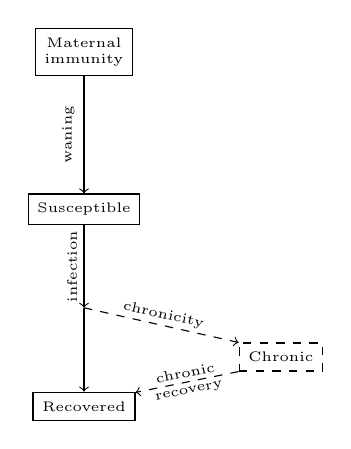
\begin{tikzpicture}[compartment/.style={rectangle, draw},
                    font=\fontsize{5pt}{6}\selectfont]
  % Compartments.
  \node at (0, 4.5) [compartment, align=center, name=MaternalImmunity] {Maternal\\immunity};
  \node at (0, 2.5) [compartment, name=Susceptible] {Susceptible};
  \node at (0, 0) [compartment, name=Recovered] {Recovered};
  \node at (2.5, 0.625) [compartment, dashed, name=Chronic] {Chronic};

  % Location for branch from Susceptible to Chronic and Recovered.
  \coordinate (recovery) at (0, 1.25);

  % Infection-related processes.
  \draw [->] (MaternalImmunity)
             to node [rotate=90, above] {waning}
             (Susceptible);
  \draw [->] (Susceptible)
             to node [rotate=90, above, yshift=-1pt] {infection}
             (recovery);
  \draw [->, dashed] (recovery)
             to node [sloped, above, yshift=-2pt] {chronicity}
             (Chronic.161);
  \draw [->] (recovery)
             to node [] {}
             (Recovered.90);
  \draw [->, dashed] (Chronic.199)
             to node [sloped, align=center] {chronic\\recovery}
             (Recovered.15);
\end{tikzpicture}
